\documentclass[english,11pt]{beamer}

\DeclareMathOperator{\Cov}{Cov}
\DeclareMathOperator{\Var}{Var}
\DeclareMathOperator{\E}{\mathbb{E}}
\DeclareMathOperator{\Proba}{\mathbb{P}}

\newcommand{\Covb}[2]{\ensuremath{\Cov\!\left[#1,#2\right]}}
\newcommand{\Eb}[1]{\ensuremath{\E\!\left[#1\right]}}
\newcommand{\Pb}[1]{\ensuremath{\Proba\!\left[#1\right]}}
\newcommand{\Varb}[1]{\ensuremath{\Var\!\left[#1\right]}}

% norm
\newcommand{\norm}[1]{\| #1 \|}

\newcommand{\indep}{\rotatebox[origin=c]{90}{$\models$}}





\usepackage{mathptmx,amsmath,amssymb,graphicx,bibentry,bbm,babel,ragged2e}

\makeatletter

\newcommand{\noun}[1]{\textsc{#1}}
\newcommand{\jitem}[1]{\item \begin{justify} #1 \end{justify} \vfill{}}
\newcommand{\sframe}[2]{\frame{\frametitle{#1} #2}}

\newenvironment{centercolumns}{\begin{columns}[c]}{\end{columns}}
%\newenvironment{jitem}{\begin{justify}\begin{itemize}}{\end{itemize}\end{justify}}









%\usetheme{Warsaw}
%\setbeamertemplate{footline}[text line]{}
%\setbeamercolor{structure}{fg=purple!50!blue, bg=purple!50!blue}
%\setbeamersize{text margin left=15pt,text margin right=15pt}




\usetheme{Boadilla}


% redefine palette
\definecolor{cybblue}{HTML}{1C6F91}


\setbeamercolor{structure}{fg=cybblue}

\setbeamercovered{transparent}


\addtobeamertemplate{title page}{%\hspace{-0.4cm}
\vspace{-0.8cm}
\hspace{-0.5cm}
%\includegraphics[height=1.2cm,width=1.2\textwidth]{template/bandeau3}\\
}{%
%\begin{textblock*}{150mm}(-1cm,-1.5cm)
%\end{textblock*}
}


\setbeamertemplate{footline}{
\hspace{0.2cm}

\includegraphics[height=0.75cm]{template/medium}
\hfill

\includegraphics[height=0.75cm]{template/eu}
\hspace{0.15cm}
\vspace{0.15cm}
}





\@ifundefined{showcaptionsetup}{}{%
 \PassOptionsToPackage{caption=false}{subfig}}
\usepackage{subfig}

\usepackage[utf8]{inputenc}
\usepackage[T1]{fontenc}


\usepackage[usenames,dvipsnames]{pstricks}
\usepackage{epsfig}



\makeatother

\begin{document}


\title{\phantom{}\bigskip\bigskip
Round Table\\\bigskip
Complexity and Knowledge of Complex Systems
}

\author{}


\institute{}


\date{Medium 2017 Conference\\\smallskip
Spatio-temporal Behavior in Complex Urban Systems\\\smallskip
17th June 2017
}


{


\setbeamertemplate{footline}{
\hspace{0.2cm}

\includegraphics[height=1cm]{template/medium}
\hfill
\textit{This Project is funded by the European Union}\hspace{0.2cm}

\includegraphics[height=1cm]{template/eu}
\hspace{0.2cm}
\vspace{0.5cm}
}


\frame{\maketitle}

}


\sframe{Contextualization}{
  % situate each presentation
  
  \footnotesize\justify
  \vspace{-0.3cm}
  
  \begin{itemize}
  \item \textbf{S. Zhou : } Patterns, Spatio-temporal Correlations and Processes as principal research questions, which understanding is enhanced by new Big Data and models.
  \item \textbf{D. Pumain : } SimpopLocal, an achievement of the evolutive Urban Theory strongly coupling empirical stylized facts with modeling experiments.
  \item \textbf{Q. Zhan : } Coupling of heterogeneous models and data, application as tool for Urban Planning.
  \item \textbf{M. Bida, C. Rozenblat and E. Swerts : } A model based on geographical and economic theories and stylized facts.
  \item \textbf{S. Wang : } An analysis of the low-carbon approach to sustainability ; proposition of a broader methodology and tools.
  \item \textbf{F. Pfaender : } Data as traces that need to be collected with elaborated tools and specific methods, used to elaborate multi-scalar empirical analyses and theoretical considerations.
  \item \textbf{Y. Yue : } Big Data on mobility used to learn stylized facts on intra-urban migration, theoretical implications for district strategies.
  \item \textbf{J. Raimbault : } A model based on theory and empirical facts.
  \end{itemize}

  
}


\sframe{Knowledge Framework}{
  % co-evolution of domains

\justify\small

\textbf{Knowledge Framework specification}

Any scientific knowledge construction on a complex system is a perspective in the sens of Giere \cite{giere2010scientific}, which is composed of knowledge contents belonging at least to necessary domains, that \emph{co-evolve}~\cite{holland2012signals} between themselves and with the other elements of the perspective, in particular the cognitive agents.

\medskip

\textbf{Necessary Knowledge Domains : }
\begin{itemize}
\item \textbf{Empirical.} Empirical knowledge of real world objects.
\item \textbf{Theoretical.} More general conceptual knowledge, implying cognitive constructions.
\item \textbf{Modeling.} The model is the formalized \emph{medium} of the scientific perspective, as diverse as Varenne's classifications of models functions~\cite{varenne2010simulations}.
\item \textbf{Data.} Raw information that has been collected.
\item \textbf{Methods.} Generic structures of knowledge production.
\item \textbf{Tools.} Proto-methods (implementation of methods) and supports of others domains.
\end{itemize}
  
}



\sframe{Knowledge Framework : illustration}{
  % 
  \centering
  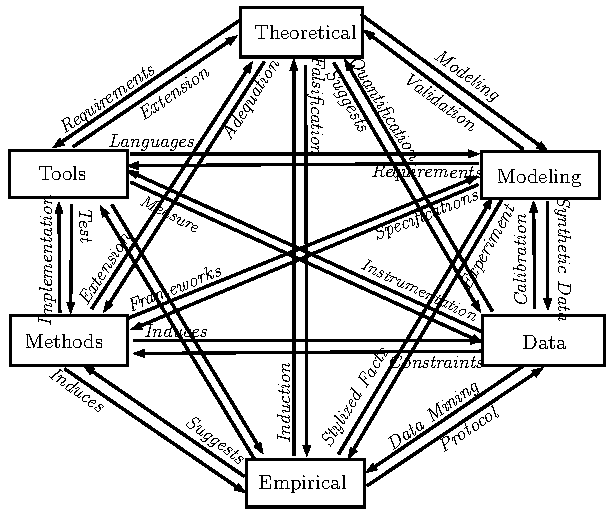
\includegraphics[height=\textheight]{figures/tqg}
}


\sframe{Questions}{

\justify

  % questions for the round table
  \textbf{Main direction : }
  
  \textit{What are the interplays between Empirical, Theories, Models, Methods, Tools and Data in your research ? What concrete benefits can be drawn/do you draw from the levels of interdependencies (high or low) ?}
  
  \bigskip
  \bigskip
  \bigskip
  
  \textbf{Corollaries : } \textit{or discuss why it shouldn't be}
  
  \begin{itemize}
  \item Role of interdisciplinarity and merging ``quantitative'' and ``qualitative'' ; difficulties to achieve these.
  \item Role and nature of complexity(ies) ; difficulty to tackle it.
  \item \textit{Bonus/Poll : Is Complex Knowledge intrinsically reflexive, and is it linked to the combination of the different natures of Complexity ?}
  \end{itemize}

  
}





%%%%%%%%%%%%%%%%%%%%%
\begin{frame}[allowframebreaks]
\frametitle{References}
\bibliographystyle{apalike}
\bibliography{/Users/Juste/Documents/ComplexSystems/CityNetwork/Biblio/Bibtex/CityNetwork}
\end{frame}
%%%%%%%%%%%%%%%%%%%%%%%%%%%%






\end{document}







